\subsection{题目描述}
\noindent Newton interpolation of:
\begin{itemize}
    \item[(1)] 10 equal spacing points of \( \cos(x) \) within \( [0, \pi] \);
    \item[(2)] 10 equal spacing points \( \frac{1}{1 + 25x^2} \) within \([-1, 1]\).
\end{itemize}
Compare the results with the cubic spline interpolation.

\subsection{程序描述}
发现等距节点在一些病态函数的插值中的确会出现Runge现象,故对有理函数\( \frac{1}{1 + 25x^2} \) 额外使用Chebyshev节点(第一类Chebyshev多项式的零点)与Leja节点进行对比研究。前者在区间\([-1, 1]\)上的分布为
\[x_k=\cos{\left(\frac{2k+1}{2n}\pi\right)},\quad k=0,\ldots,n-1,\]
用于插值\((n-1)\)阶多项式,它们同时也是单位圆上的等距点在\([-1, 1]\)上的投影,可以使得拉格朗日余项
\[f(x)-P_{n-1}(x)=\frac{f^{(n)}(\xi)}{n!}\prod_{i=1}^n(x-x_i)\]
中的\(\max_{x\in[-1,1]}\Big|\prod_{i=1}^n(x-x_i)\Big|\)最小化,故最终在\([-1, 1]\)上的插值余项满足
\[|f(x)-P_{n-1}(x)|\leq\frac1{2^{n-1}n!}\max_{\xi\in[-1,1]}\left|f^{(n)}(\xi)\right|.\]上述理论可以拓展到任意长度的区间\([a,b]\),仅需使用相应的Chebyshev节点
\[x_k=\frac{(a+b)}2+\frac{(b-a)}2\cos\left(\frac{2k+1}{2n}\pi\right),\quad k=0,\ldots,n-1.\]

在思考拓展题的舍入误差时,联想到牛顿插值法的数值稳定性可能的确受到节点顺序的影响。一篇满是奇怪符号和不等式的论文\footnote{Camargo, A.P. (2020). On the numerical stability of Newton’s formula for Lagrange interpolation. \textit{Journal of Computational and Applied Mathematics}, 365.\href{https://doi.org/10.1016/j.cam.2019.112369}{10.1016/j.cam.2019.112369}}
告诉我,可以使用Lebesgue常数来衡量重心形式拉格朗日插值的数值稳定性:
\[
\Lambda\left(\mathbf{x}\right):=max_{x\in\left[a,b\right]}\left(\sum_{i=0}^n\prod_{k\neq i}^n\left|\frac{x-x_k}{x_i-x_k}\right|\right)
\]
对于牛顿插值,该文给出了三类上界,公式与推导很催眠,我选择使用两个更病态的函数进行了数值实验,详见拓展题。使用的另一套节点是Leja节点,首先定一个初始节点(通常为峰值点),再按照满足如下条件增加节点,使得每个节点“尽可能离之前的点远”
\[
|x_{k+1} - x_0| \cdot |x_{k+1} - x_1| \cdot \dots \cdot |x_{k+1} - x_k| = \max_{x \in [a,b]} \prod_{i=0}^{k} |x - x_i|, \quad k = 0, 1, \dots, n-1
\]
一篇看起来符号少些但逻辑不是很清楚的文章\footnote{Carnicer, J.M., Khiar, Y. \& Peña, J.M. (2019). Central orderings for the Newton interpolation formula. \textit{Bit Numer Math}, 59, 371–386.\href{https://doi.org/10.1007/s10543-018-00743-2}{10.1007/s10543-018-00743-2}}告诉我,使用中心序的Leja节点可以使得牛顿插值法的数值稳定性更好,但实验结果好像不符(倒是和三次插值配合很好),可能是代码问题,也可能是优化方法并不普适。为了更好利用\texttt{numpy}库的向量化操作,本程序构建完牛顿差商表计算给定点值时,使用了Horner's Rule,即迭代计算
\[
\begin{aligned}
P_n(x) &= f[x_0] + f[x_1, x_0](x - x_0) + f[x_2, x_1, x_0](x - x_0)(x - x_1) + \cdots\\
&+ f[x_n, x_{n-1}, \dots, x_0](x - x_0)(x - x_1)\dots(x - x_{n-1}) \\
&= f[x_0] + (x - x_0) \left( f[x_1, x_0] + (x - x_1) \left( f[x_2, x_1, x_0] + \cdots + (x - x_{n-1}) f[x_n, x_{n-1}, \dots, x_0] \right) \right)
\end{aligned}
\]
将$n(n+1)/2$次乘法降至$n$次。似乎还有一种古老的Neville's Algorithm\footnote{详见\textit{Numerical Recipes $\S 3.1$}},可以在局部点加速收敛。

在三次插值部分使用了Thomas算法来快速求解条状矩阵以提高数值稳定性,剩下的大段代码都是GPT的绘图美化工程,它真的很尽职。最终插值结果详见下文结果示例。请在本程序目录使用\ccmd{python -u newton\_cubic.py}运行数值实验,需安装\texttt{numpy}和\texttt{matplotlib}库。

\subsection{伪代码}
\begin{algorithm}[H]
    \caption{Leja Node Generation}
    \KwIn{$a(float)$, $b(float)$, $n(int)$, $m(int)$, $f(function)$}
    \KwOut{$nodes(array, shape=n)$}

        $x(array, shape=m) \leftarrow$ discretize interval $[a,b]$ into $m$ points
        $nodes(array, shape=n)$  \tcp*[r]{Initialize array for Leja nodes}
        nodes[0] $\leftarrow x[\arg\max(|f(x)|)]$  \tcp*[r]{Select the point where $|f(x)|$ is maximum as the first node}
        \For{$i \leftarrow 1$ \KwTo $n-1$}{
            $distances[j] \leftarrow \min(|x[j] - \text{nodes}[k]|)$ for $k=0, \dots, i-1$ and $j=0, \dots, m-1$  \tcp*[r]{Compute minimum distance from each point to the current nodes}
            nodes[$i$] $\leftarrow x[\arg\max(distances)]$  \tcp*[r]{Select the point with the maximum distance as the next node}
        }
        \KwRet{nodes}  \tcp*[r]{Return the array of Leja nodes}
\end{algorithm}

\begin{algorithm}[H]
    \caption{Newton's Divided Difference Method}
    \KwIn{$x(array, shape=n+1)$, $y(array, shape=n+1)$}
    \KwOut{$coef(array, shape=n+1)$}
        $n \leftarrow$ length($y$) - 1  \tcp*[r]{Determine the degree of the polynomial}
        $coef(array, shape=n+1) \leftarrow y$  \tcp*[r]{Initialize coefficients with $y$ values}
        \For{$j \leftarrow 1$ \KwTo $n$}{
            \For{$i \leftarrow n$ \KwTo $j$}{
                coef[$i$] $\leftarrow \frac{\text{coef}[i] - \text{coef}[i-1]}{x[i] - x[i-j]}$  \tcp*[r]{Compute divided differences}
            }
        }
        \KwRet{coef}  \tcp*[r]{Return the array of divided difference coefficients}
    \end{algorithm}

    \begin{algorithm}[H]
        \caption{Cubic Spline Interpolation}
        \KwIn{$x(array, shape=n+1)$, $y(array, shape=n+1)$}
        \KwOut{$a(array, shape=n)$, $b(array, shape=n)$, $c(array, shape=n+1)$, $d(array, shape=n)$}
        \SetKwFunction{SolveTridiagonal}{SolveTridiagonal}
            $h[i] \leftarrow x[i+1] - x[i]$ for $i=0,\dots,n-1$ 
            $A[0,0] \leftarrow 1, A[n,n] \leftarrow 1$  \tcp*[r]{Set boundary conditions}
            \For{$i \leftarrow 1$ \KwTo $n-1$}{
                $A[i, i-1] \leftarrow h[i-1], A[i, i] \leftarrow 2(h[i-1] + h[i]), A[i, i+1] \leftarrow h[i]$  \tcp*[r]{Fill tridiagonal matrix}
                $b[i] \leftarrow 3 \left(\frac{y[i+1] - y[i]}{h[i]} - \frac{y[i] - y[i-1]}{h[i-1]}\right)$  \tcp*[r]{Compute right-hand side vector for spline system}
            }
            $c \leftarrow$ \SolveTridiagonal{$A, b$}  \tcp*[r]{Solve for $c$ coefficients using the tridiagonal matrix}
            
            \For{$i \leftarrow 0$ \KwTo $n-1$}{
                $b[i] \leftarrow \frac{y[i+1] - y[i]}{h[i]} - \frac{h[i]}{3} (2c[i] + c[i+1])$ ; $d[i] \leftarrow \frac{c[i+1] - c[i]}{3h[i]}$  
            }
            $a \leftarrow y[0:n]$  \tcp*[r]{Assign $a$ coefficients from $y$ values}
            \KwRet{$a, b, c, d$}  \tcp*[r]{Return the spline coefficients}
        \end{algorithm}

        \begin{algorithm}[H]
            \caption{Solve Tridiagonal System (Thomas Algorithm)}
            \KwIn{$A(array, shape=(n+1, n+1))$, $b(array, shape=n+1)$}
            \KwOut{$x(array, shape=n+1)$}
                $c'[0] \leftarrow \frac{A[0,1]}{A[0,0]}$, $d'[0] \leftarrow \frac{b[0]}{A[0,0]}$  \tcp*[r]{Initial forward sweep for $c'$ and $d'$}
                \For{$i \leftarrow 1$ \KwTo $n-1$}{
                    $denom \leftarrow A[i,i] - A[i,i-1] \cdot c'[i-1]$  \tcp*[r]{Calculate denominator for row $i$}
                    $c'[i] \leftarrow \frac{A[i,i+1]}{denom}$, $d'[i] \leftarrow \frac{b[i] - A[i,i-1] \cdot d'[i-1]}{denom}$  \tcp*[r]{Update $c'$ and $d'$ for current row}
                }
                $d'[n] \leftarrow \frac{b[n] - A[n,n-1] \cdot d'[n-1]}{A[n,n] - A[n,n-1] \cdot c'[n-1]}$ ;  $x[n] \leftarrow d'[n]$  \tcp*[r]{Final update for $d'[n]$}
                \For{$i \leftarrow n-1$ \KwTo 0}{
                    $x[i] \leftarrow d'[i] - c'[i] \cdot x[i+1]$  \tcp*[r]{Back substitution step for $x[i]$}
                }
                \KwRet{$x$}  \tcp*[r]{Return the solution array $x$}
            \end{algorithm}

\subsection{结果示例}
\begin{figure}[H]
    \centering
    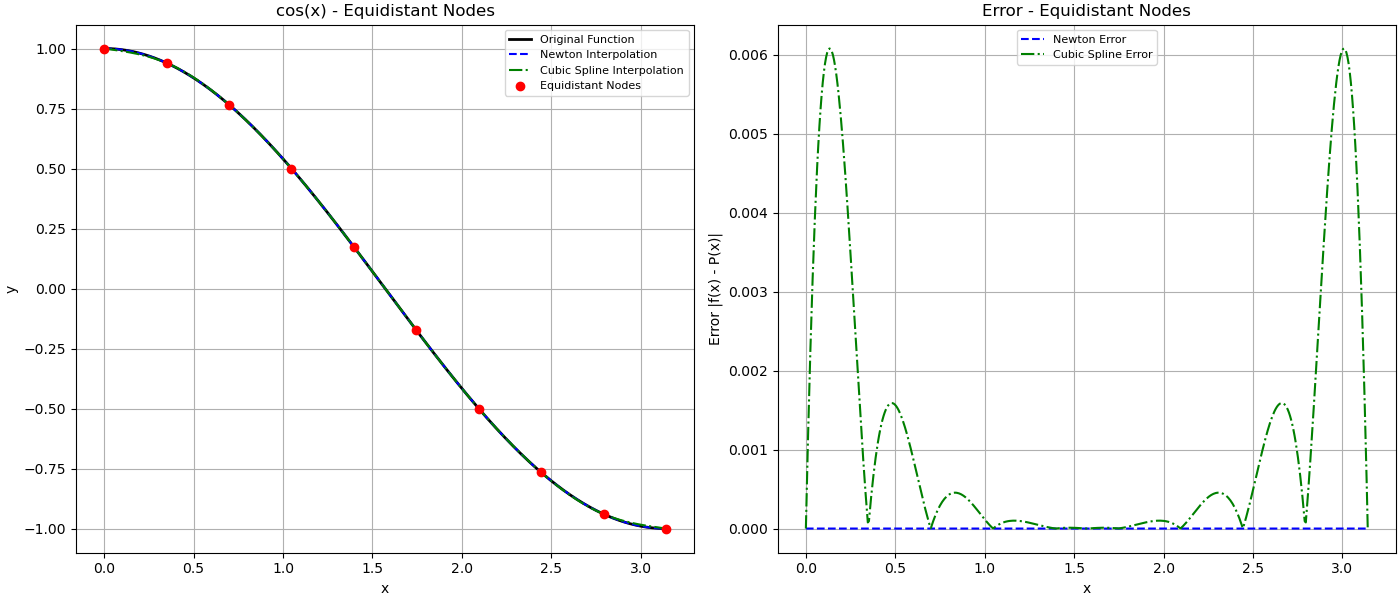
\includegraphics[width=1.0\textwidth]{Problem_1/figs/cos.png}
    \caption{$cos(x)$插值效果对比}
\end{figure}

\begin{figure}[H]
    \centering
    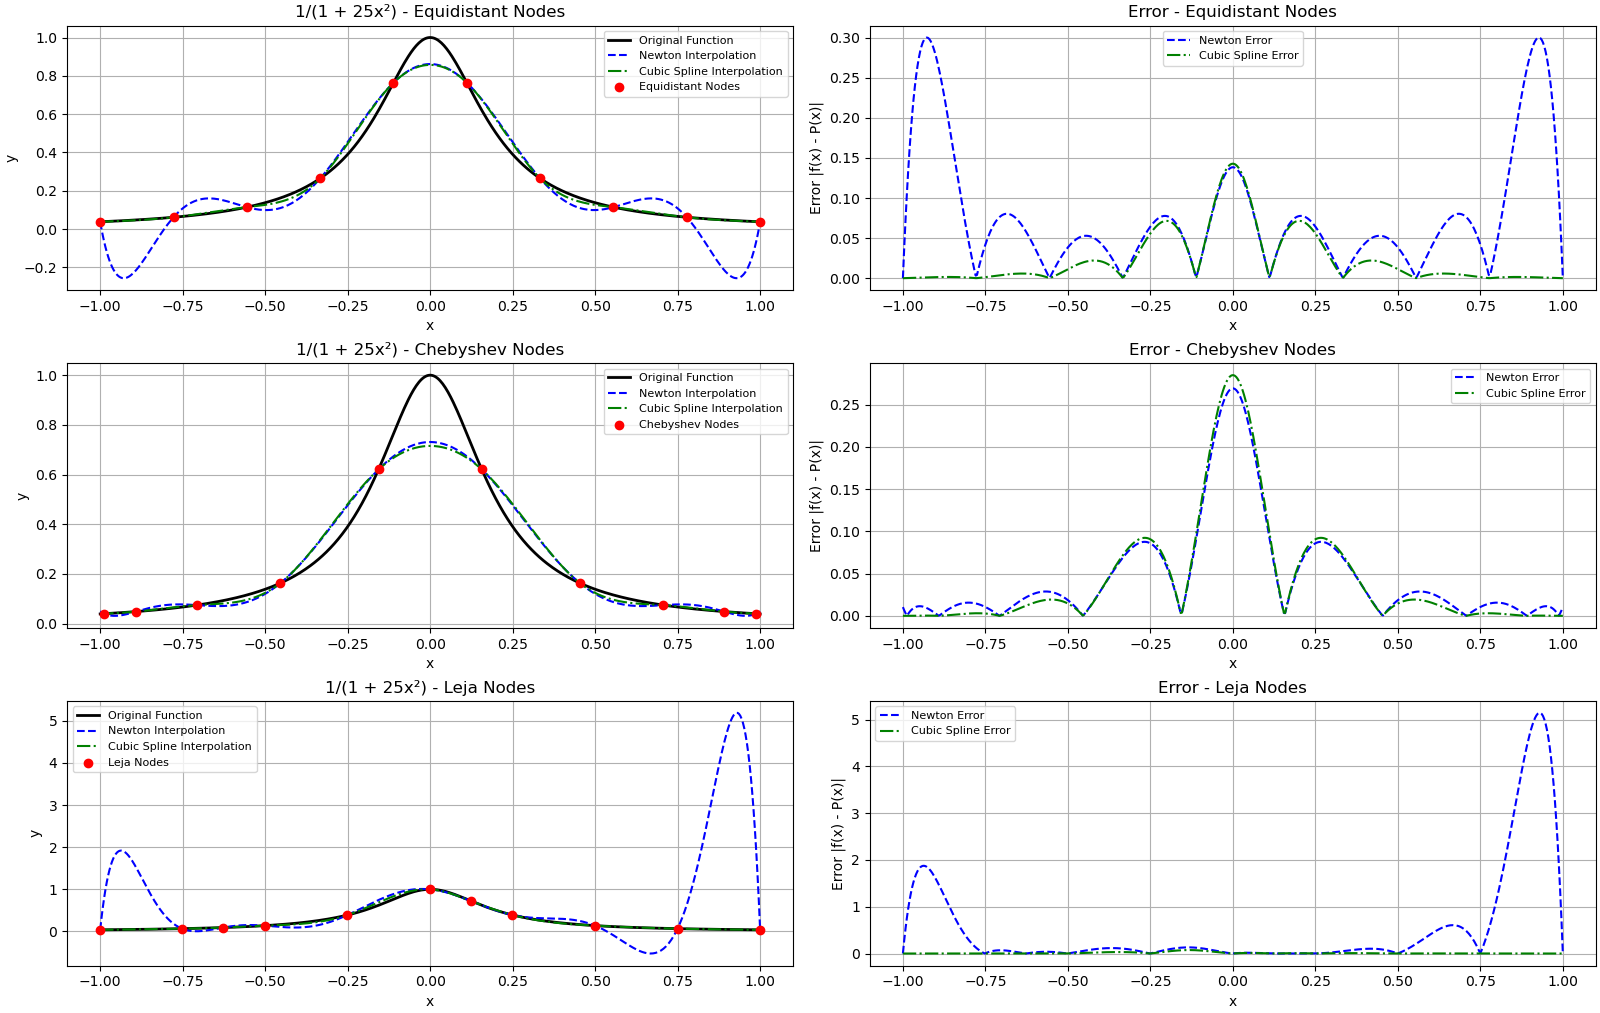
\includegraphics[width=1.0\textwidth]{Problem_1/figs/rational.png}
    \caption{$\frac{1}{1+25x^2}$插值效果对比}
\end{figure}

\begin{figure}[H]
    \centering
    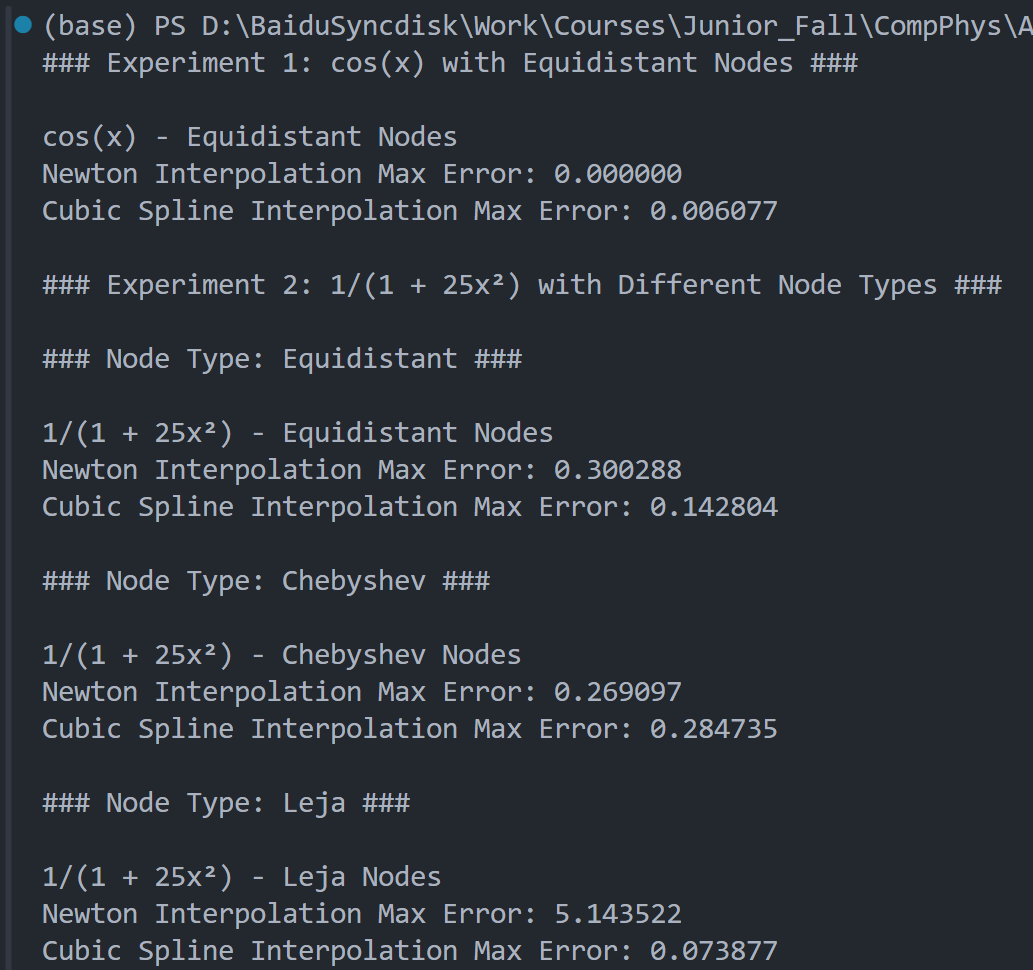
\includegraphics[width=0.8\textwidth]{Problem_1/figs/result.png}
    \caption{终端输出}
\end{figure}
